\begin{figure}[htbp]
\centering
\resizebox{0.98\linewidth}{!}{%
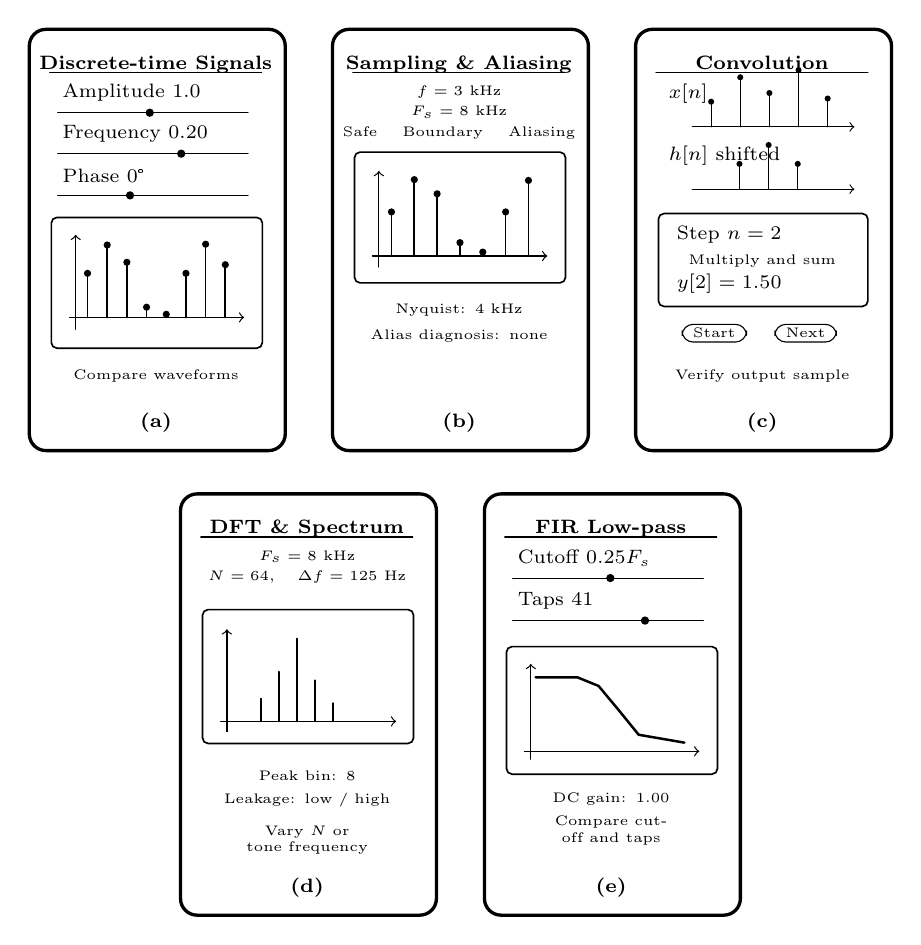
\begin{tikzpicture}[font=\sffamily, line cap=round, line join=round]

\tikzset{
  handset/.style={draw, very thick, rounded corners=6pt, minimum width=3.25cm, minimum height=5.35cm, inner sep=0pt},
  card/.style={draw, rounded corners=2pt, line width=0.6pt},
  tinylabel/.style={font=\scriptsize},
  compactlabel/.style={font=\tiny, align=center, text width=2.45cm},
  paneltitle/.style={font=\bfseries\scriptsize, align=center}
}

% ==================== (a) Signals ====================
\begin{scope}[shift={(0,5.9)}]
  \node[handset, anchor=north west] at (0,0) {};
  \node[paneltitle, anchor=north] at (1.625,-0.23) {Discrete-time Signals};
  \draw[line width=0.5pt] (0.28,-0.57) -- (2.97,-0.57);
  \node[tinylabel, anchor=west] at (0.32,-0.83) {Amplitude  1.0};
  \draw (0.38,-1.08) -- (2.80,-1.08); \fill (1.55,-1.08) circle (1.5pt);
  \node[tinylabel, anchor=west] at (0.32,-1.35) {Frequency  0.20};
  \draw (0.38,-1.60) -- (2.80,-1.60); \fill (1.95,-1.60) circle (1.5pt);
  \node[tinylabel, anchor=west] at (0.32,-1.88) {Phase  0\textdegree};
  \draw (0.38,-2.13) -- (2.80,-2.13); \fill (1.30,-2.13) circle (1.5pt);
  \node[card, minimum width=2.68cm, minimum height=1.66cm, anchor=north west] at (0.29,-2.40) {};
  \draw[->,line width=0.45pt] (0.53,-3.68) -- (2.75,-3.68);
  \draw[->,line width=0.45pt] (0.61,-3.83) -- (0.61,-2.63);
  \foreach \x/\y in {0.76/-3.12,1.01/-2.76,1.26/-2.98,1.51/-3.55,1.76/-3.64,2.01/-3.12,2.26/-2.75,2.51/-3.01} {
    \draw[line width=0.6pt] (\x,-3.68) -- (\x,\y); \fill (\x,\y) circle (1.3pt);
  }
  \node[compactlabel] at (1.63,-4.42) {Compare waveforms};
  \node[font=\bfseries\scriptsize] at (1.63,-5.02) {(a)};
\end{scope}

% ==================== (b) Sampling ====================
\begin{scope}[shift={(3.85,5.9)}]
  \node[handset, anchor=north west] at (0,0) {};
  \node[paneltitle, anchor=north] at (1.625,-0.23) {Sampling \& Aliasing};
  \draw[line width=0.5pt] (0.28,-0.57) -- (2.97,-0.57);
  \node[font=\tiny, align=center] at (1.63,-0.82) {$f=3$ kHz};
  \node[font=\tiny, align=center] at (1.63,-1.07) {$F_s=8$ kHz};
  \node[font=\tiny, align=center] at (1.63,-1.34) {Safe \quad Boundary \quad Aliasing};
  \node[card, minimum width=2.68cm, minimum height=1.66cm, anchor=north west] at (0.29,-1.57) {};
  \draw[->,line width=0.45pt] (0.53,-2.90) -- (2.75,-2.90);
  \draw[->,line width=0.45pt] (0.61,-3.04) -- (0.61,-1.82);
  \foreach \x/\y in {0.77/-2.34,1.06/-1.93,1.35/-2.11,1.64/-2.73,1.93/-2.85,2.22/-2.34,2.51/-1.94} {
    \draw[line width=0.6pt] (\x,-2.90) -- (\x,\y); \fill (\x,\y) circle (1.3pt);
  }
  \node[compactlabel] at (1.63,-3.59) {Nyquist: 4 kHz};
  \node[compactlabel] at (1.63,-3.91) {Alias diagnosis: none};
  \node[font=\bfseries\scriptsize] at (1.63,-5.02) {(b)};
\end{scope}

% ==================== (c) Convolution ====================
\begin{scope}[shift={(7.70,5.9)}]
  \node[handset, anchor=north west] at (0,0) {};
  \node[paneltitle, anchor=north] at (1.625,-0.23) {Convolution};
  \draw[line width=0.5pt] (0.28,-0.57) -- (2.97,-0.57);
  \node[tinylabel, anchor=west] at (0.32,-0.84) {$x[n]$};
  \draw[->,line width=0.4pt] (0.74,-1.26) -- (2.80,-1.26);
  \foreach \x/\h in {0.98/0.32,1.35/0.63,1.72/0.43,2.09/0.72,2.46/0.36}{\draw (\x,-1.26)--(\x,{-1.26+\h});\fill (\x,{-1.26+\h}) circle (1.1pt);}
  \node[tinylabel, anchor=west] at (0.32,-1.63) {$h[n]$ shifted};
  \draw[->,line width=0.4pt] (0.74,-2.05) -- (2.80,-2.05);
  \foreach \x/\h in {1.34/0.32,1.71/0.56,2.08/0.32}{\draw (\x,-2.05)--(\x,{-2.05+\h});\fill (\x,{-2.05+\h}) circle (1.1pt);}
  \node[card, minimum width=2.66cm, minimum height=1.18cm, anchor=north west] at (0.30,-2.35) {};
  \node[tinylabel, anchor=west] at (0.42,-2.63) {Step $n=2$};
  \node[compactlabel] at (1.63,-2.96) {Multiply and sum};
  \node[tinylabel, anchor=west] at (0.42,-3.25) {$y[2]=1.50$};
  \node[font=\tiny, draw, rounded corners=4pt, inner xsep=4pt, inner ysep=1.5pt] at (1.02,-3.88) {Start};
  \node[font=\tiny, draw, rounded corners=4pt, inner xsep=4pt, inner ysep=1.5pt] at (2.18,-3.88) {Next};
  \node[compactlabel] at (1.63,-4.42) {Verify output sample};
  \node[font=\bfseries\scriptsize] at (1.63,-5.02) {(c)};
\end{scope}

% ==================== (d) DFT ====================
\begin{scope}[shift={(1.92,0)}]
  \node[handset, anchor=north west] at (0,0) {};
  \node[paneltitle, anchor=north] at (1.625,-0.23) {DFT \& Spectrum};
  \draw[line width=0.5pt] (0.28,-0.57) -- (2.97,-0.57);
  \node[font=\tiny, align=center] at (1.63,-0.82) {$F_s=8$ kHz};
  \node[font=\tiny, align=center] at (1.63,-1.08) {$N=64,\quad \Delta f=125$ Hz};
  \node[card, minimum width=2.68cm, minimum height=1.70cm, anchor=north west] at (0.29,-1.48) {};
  \draw[->,line width=0.45pt] (0.53,-2.91) -- (2.76,-2.91);
  \draw[->,line width=0.45pt] (0.61,-3.04) -- (0.61,-1.74);
  \draw[line width=0.75pt] (1.04,-2.91)--(1.04,-2.62);
  \draw[line width=0.75pt] (1.27,-2.91)--(1.27,-2.28);
  \draw[line width=0.75pt] (1.50,-2.91)--(1.50,-1.86);
  \draw[line width=0.75pt] (1.73,-2.91)--(1.73,-2.39);
  \draw[line width=0.75pt] (1.96,-2.91)--(1.96,-2.68);
  \node[compactlabel] at (1.63,-3.60) {Peak bin: 8};
  \node[compactlabel] at (1.63,-3.91) {Leakage: low / high};
  \node[compactlabel] at (1.63,-4.42) {Vary $N$ or tone frequency};
  \node[font=\bfseries\scriptsize] at (1.63,-5.02) {(d)};
\end{scope}

% ==================== (e) FIR ====================
\begin{scope}[shift={(5.78,0)}]
  \node[handset, anchor=north west] at (0,0) {};
  \node[paneltitle, anchor=north] at (1.625,-0.23) {FIR Low-pass};
  \draw[line width=0.5pt] (0.28,-0.57) -- (2.97,-0.57);
  \node[tinylabel, anchor=west] at (0.32,-0.84) {Cutoff  $0.25F_s$};
  \draw (0.38,-1.09) -- (2.80,-1.09); \fill (1.62,-1.09) circle (1.5pt);
  \node[tinylabel, anchor=west] at (0.32,-1.38) {Taps  41};
  \draw (0.38,-1.63) -- (2.80,-1.63); \fill (2.06,-1.63) circle (1.5pt);
  \node[card, minimum width=2.68cm, minimum height=1.62cm, anchor=north west] at (0.29,-1.95) {};
  \draw[->,line width=0.45pt] (0.53,-3.29) -- (2.75,-3.29);
  \draw[->,line width=0.45pt] (0.61,-3.39) -- (0.61,-2.18);
  \draw[line width=0.9pt] (0.67,-2.35) -- (1.20,-2.35) -- (1.47,-2.46) -- (1.72,-2.76) -- (1.98,-3.08) -- (2.56,-3.18);
  \node[compactlabel] at (1.63,-3.90) {DC gain: 1.00};
  \node[compactlabel] at (1.63,-4.30) {Compare cutoff and taps};
  \node[font=\bfseries\scriptsize] at (1.63,-5.02) {(e)};
\end{scope}

\end{tikzpicture}%
}
\caption{Representative DSP-Lab interface overview. The schematic panels summarize the common mobile interaction pattern across the five learning modules: parameter adjustment, immediate graphical or numerical feedback, guided comparison, and short explanation. (a) discrete-time signals; (b) sampling and aliasing; (c) convolution; (d) DFT and spectrum; and (e) FIR filtering.}
\label{fig:app-interface-overview}
\end{figure}
